% Preamble
% ---
\documentclass{article}

% Packages
% ---
\usepackage{amsmath} % Advanced math typesetting
\usepackage[utf8]{inputenc} % Unicode support (Umlauts etc.)
\usepackage{hyperref} % Add a link to your document
\hypersetup{
colorlinks=true,
linkcolor=black,
filecolor=black,
citecolor=blue,
urlcolor=blue,
}
\usepackage{graphicx} % Add pictures to your document
\usepackage{listings} % Source code formatting and highlighting
\usepackage{framed} % Source code formatting and highlighting
\usepackage{appendix} % Source code formatting and highlighting
\usepackage{csquotes} % Pretty quotes
\usepackage[letterpaper, portrait, margin=1in]{geometry}
\usepackage{multicol}
\usepackage{parskip}
\usepackage{tikz}
\usetikzlibrary{arrows.meta, positioning}
\usepackage{ragged2e}
\usepackage[table]{xcolor} % Enables coloring in tables
\usepackage{tabularx}
\addtolength{\skip\footins}{10pt}
\usepackage{indentfirst}
\graphicspath{ {images/} }

\title {Proof of Perfect White Paper}

\author{
Joel Carter,
Arie Trouw,
Matt Jones,
Jordan Trouw
\thanks{XYO - \texttt{arie.trouw@xyo.network, joel.carter@xyo.network, matt.jones@xyo.network, jordan.trouw@xyo.network}}
}

\date{March 2025}

\begin{document}
\maketitle

\begin{center}
  \line(1,0){50}
\end{center}

%Abstract Section
\begin{abstract}
  In areas of life where multiple parties interact to achieve an ideal outcome, from those as mundane as choosing where to go for dinner to those as weighty as voting on elected officials, the need for a clear and deterministic distributed consensus algorithm underlies the stability of the system. This need, and the associated solutions, have recently been of pioneering interest in the blockchain space.
  \begin{center}
    \line(1,0){50}
  \end{center}
\end{abstract}

\section{Current Landscape}
There exist several recognized and widely adopted solutions for coming to
distributed consensus in the blockchain space.

\subsection{Proof of Work (PoW)}
\subsubsection{Benefits}
Revolutionized decentralized consensus by using computational puzzles to secure
networks, ensuring trust without a central authority.
\subsubsection{Limitations}
\begin{itemize}
  \item High energy consumption.
  \item Slow transaction speeds.
  \item Centralization risks due to mining pools.
  \item Vulnerability to 51\% attacks.
  \item Risk of a single entity controlling the network with enough compute power.
\end{itemize}

\subsection{Proof of Stake (PoS)}
\subsubsection{Benefits}
Pioneered a more energy-efficient consensus model by leveraging stakeholders’
assets, reducing energy use and offering faster transaction speeds. Encourages
diversification of producers through random shuffling algorithms.
\subsubsection{Limitations}
\begin{itemize}
  \item \enquote{Nothing at stake} problem.
  \item Centralization risk with large stakeholders.
  \item Vulnerability to long-range attacks.
  \item Challenges in ensuring network security without high energy costs.
\end{itemize}

\section{Characteristics of an Ideal Algorithm}

Given the existing shortcomings of the current consensus algorithms it becomes
advantageous to envision a more ideal algorithm that maintains the guarantees
of the existing solutions while addressing their shortcomings. Paramount to any
distributed consensus algorithm for a blockchain is the ability to, given two
equally valid uncles, choose the best one. Moreover, for an algorithm to be
ideal it must not just meet the goal of consensus or even meet it well, but it
must be antifragile-–resilient and gaining in positive attributes--when subject
to the hostile entropy of the real world use cases it is subject to. The table
below lists several metrics across which an algorithm which arrives at that end
might be evaluated.

  {
    \hyphenpenalty=10000\exhyphenpenalty=10000
    \renewcommand{\arraystretch}{1.5}
    \begin{table}[h]
      \centering
      \begin{tabular}{|>{\RaggedRight\arraybackslash}p{3.5cm}|>{\RaggedRight\arraybackslash}p{3.5cm}|>{\RaggedRight\arraybackslash}p{3.5cm}|>{\RaggedRight\arraybackslash}p{3.5cm}|}
        \hline
        \rowcolor{lightgray}
        \textbf{Metric}       & \textbf{Good}                                                                          & \textbf{Better}                                                                                                              & \textbf{Best}                                                                                                    \\
        \hline
        Consensus Mechanism   & Independently verifiable                                                               & Simple to calculate                                                                                                          & Hard to manipulate                                                                                               \\
        \hline
        CAP Theorem Balance   & Chooses a balance of Consistency, Atomicity, and Partition Tolerance                   & Has an ideal balance for the network participants across conditions                                                          & Network partitions introduce minimal disruption due to constantly choosing best uncle, even when not partitioned \\
        \hline
        Scale                 & Does not fail as the network scales                                                    & Handles all reasonable scales across which the network will encounter without degrading in performance or increasing in cost & Gains in efficiency, robustness, \& decentralization as the network scales                                       \\
        \hline
        Network Participation & Allows users of a sufficient threshold (financial, technological, etc.) to participate & Allows all users to participate                                                                                              & Encourages decentralization and variety of participants at the protocol level                                    \\
        \hline
      \end{tabular}
      \caption{Tiered Comparison of Sample Blockchain Characteristics}
    \end{table}
  }

\subsection{For a Single Block}
Towards the goal of arriving at consensus, given N number of potential blocks
for inclusion in the blockchain which are all individually valid, it becomes
desirable to have a mechanism for comparing blocks to provide an unbiased and
impartial way for determining whether a block is more ideal for inclusion in
the blockchain. This provides a tie-breaker of sorts when deciding which
previous blocks to build on for block producers and an evaluation criteria for
validators to decide which of the candidate chains to work on as it likely has
the highest probability of being accepted. Existing mechanisms for this are the
first produced block in PoW or the block produced by the next elected producer
in PoS.

Of paramount importance to selecting the next block is the effect that a single
block can have in influencing the direction of a blockchain which leads to the
following maxims.

\begin{itemize}
  \item It is not acceptable for the next block in a blockchain to have an outsized
        influence on the chain, such as forcing an uncle to be accepted as the new
        chain, as it allows a single network actor such a block producer with
        sufficient computational power to manipulate the entire network.
  \item It is permissible for the cumulative effect of older blocks, which are already
        included in the chain to have an outsized influence on the future of the chain
        so long as there was no way during the production of the blocks for any of the
        network actors to have known they would influence events.
\end{itemize}

A simple but robust accounting system could be derived for a single block
giving each potential block a score such that the block score is the weighted
sum of the positive aspects to be encouraged minus the weighted sums of the
negative aspects we wish to discourage. For example, for a blockchain which
that only desires to encourage decentralization, the following would apply.

\[
  \mathit{Score}_{\mathit{Block}} = \mathit{Score}_{\mathit{Decentralization}} - \mathit{Score}_{\mathit{Centralization}}
\]

Combining multiple desired/undesired traits with respective weights gives the
following.

\[
  \mathit{Score}_{\mathit{Block}} = \sum_{i \in Q} \mathit{Weight}_i (\mathit{Score}_i - \mathit{Score}_{i'})
\]

{
\hyphenpenalty=10000\exhyphenpenalty=10000
\renewcommand{\arraystretch}{1.5}
\begin{table}[h]
  \centering
  \begin{tabular}{|>{\RaggedRight\arraybackslash}l|>{\RaggedRight\arraybackslash}p{10cm}|}
    \hline
    Q                              & Set of all qualities to emphasize                                          \\
    \hline
    $\mathit{Score}_{\mathit{i}}$  & The measure to which the block exhibits the desired quality                \\
    \hline
    $\mathit{Score}_{\mathit{i'}}$ & The measure to which the block exhibits the inverse of the desired quality \\
    \hline
    $\mathit{Weight}_{\mathit{i}}$ & The weight at which the quality should be emphasized                       \\
    \hline
  \end{tabular}
  \caption{Single Block Scoring Key}
\end{table}
}

\subsection{Across Multiple Blocks}

\begin{quote}
  \enquote{The test of a first-rate intelligence is the ability to hold two opposed ideas in the mind at the same time, and still retain the ability to function.}

  \hfill — F. Scott Fitzgerald, The Crack-Up
\end{quote}

Building on individual block evaluation, it becomes necessary to have a method
of evaluating N potential chains which are all independently valid for
determining which chain is more ideal for defining and furthering the
blockchain. Mechanisms such as Proof of Work (PoW) or Proof of Stake (PoS)
allow for comparing multiple chains to provide an unbiased and impartial means
for achieving this but have some shortcomings as address previously.

One of the most ubiquitous and well proven models for arriving at a desired
state across discrete data, like blocks in a blockchain, is a Control System.
Control systems, of the architecture shown in Figure~\ref{fig:control_system},
exist for applications as varied as thermostats to self-driving vehicles and
can be adapted to model blockchain consensus.

\begin{figure}[h]
  \centering
  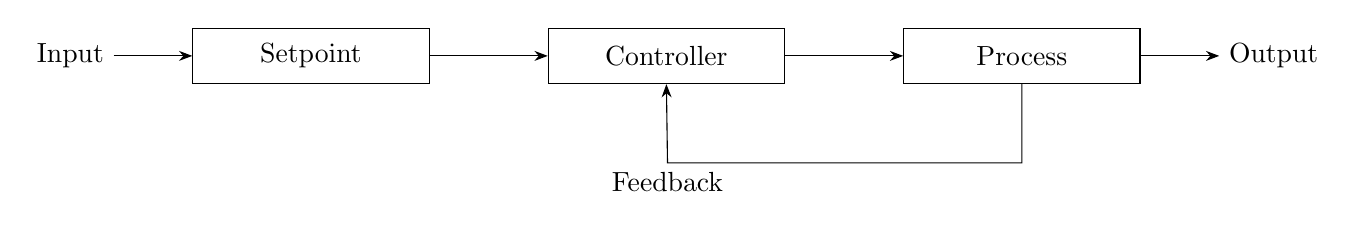
\begin{tikzpicture}[
      block/.style={draw, rectangle, minimum height=2em, minimum width=3cm},
      >=Stealth
    ]

    % Nodes
    \node (input) at (0,0) {Input};
    \node[block, right=1cm of input] (setpoint) {Setpoint};
    \node[block, right=1.5cm of setpoint] (controller) {Controller};
    \node[block, right=1.5cm of controller] (process) {Process};
    \node[right=1cm of process] (output) {Output};

    % Arrows
    \draw[->] (input) -- (setpoint);
    \draw[->] (setpoint) -- (controller);
    \draw[->] (controller) -- (process);
    \draw[->] (process) -- (output);

    % Feedback loop
    \draw[->] (process.south) -- ++(0,-1) node[below] {}
    -- ++(-4.5,0) node[below] (fbtext) {Feedback}
    -- (controller.south);

  \end{tikzpicture}
  \caption{A Control System}
  \label{fig:control_system}
\end{figure}

A familiar Control System is a car’s shocks and struts which work together to
absorb bumps and steady the suspension, keeping the ride smooth by controlling
how much the vehicle moves and how quickly it settles. In a similar fashion, a
blockchain can be viewed as a continuously correcting system across which
producers, users, and cryptographic algorithms constantly interact with each
other to achieve consensus. For PoW chains the Control System can be modeled as
the simplified Controls System in Table~\ref{fig:pow_control_system}.

{
\hyphenpenalty=10000\exhyphenpenalty=10000
\renewcommand{\arraystretch}{1.5}
\begin{table}[h]
  \centering
  \begin{tabular}{|>{\RaggedRight\arraybackslash}l|>{\RaggedRight\arraybackslash}p{10cm}|}
    \hline
    Input      & Difficulty Level                                \\
    \hline
    Setpoint   & Block interval                                  \\
    \hline
    Controller & Difficulty adjustment                           \\
    \hline
    Process    & Miners generating blocks                        \\
    \hline
    Output     & Actual time to mine next block                  \\
    \hline
    Feedback   & Difference between actual \& desired block time \\
    \hline
  \end{tabular}
  \caption{PoW Control System}
  \label{fig:pow_control_system}
\end{table}
}

For PoS chains the Control System becomes more complex implementing multiple
logical Control Systems for things like network throughput, gas economics, etc.
PoS chain Control Systems, while more complex than those of PoS, underscore the
need for optimizing the for more than just a single blockchain metric.

An ideal Control System for a blockchain would produce an optimal chain by
continuously evaluating and controlling for multiple metrics while also
including mechanisms to prevent participants from manipulating or negatively
influencing the blockchain.

\begin{itemize}
  \item Prevent immediate correction (limit influence of a single block)
  \item Amplify/attenuate across multiple blocks to achieve desired setpoint
  \item Use randomness and decentralization to prevent deterministic attacks
\end{itemize}

\section{Features}
\subsection{Dampening Effect}
Longer than just previous block
\subsection{Amplify/Attenuate}
\[
  \sum_{\mathit{W} - \mathit{N}}^{\mathit{N}} \mathit{N} \, \mathit{x}_{\mathit{i}}
\]

\section{Proof of Perfect}
\[
  \sum_{i = \mathit{W} - \mathit{N}}^{\mathit{N}}
  ((\mathit{P} - \mathit{N}) \, {(\mathit{W} - \mathit{i})}) / (\mathit{W} - \mathit{i})
\]

Weighted contributions to rolling average with past counting for more Emphasize
the value of randomness to prevent deterministic attacks

notes on - Kalman filters as options - Bayesian Probabilistic feedback - or
even an appropriately bounded Markov models

\end{document}